\documentclass[lesson_slides]{subfiles}
%\usepackage{natbib}
\usepackage{graphicx}
% \graphicspath{ {./images/} }
\usepackage{enumerate}
\usepackage{soul} % strike text
\usepackage{pifont} % for ding
\usepackage{float} % keeps tables in the exact position they occupy in the code
\usepackage{xcolor} % text colour
\usepackage{gb4e} % leave last

\begin{document}
%%=-=-=-=-=-=-=-=-=-=-=-=-=-=-=-=-=-=-=-=-=-=-=-=-=-=-=-=-=-=-=-=-=-=-=-=-=-=-=-=
%   FRAME START   -=-=-=-=-=-=-=-=-=-=-=-=-=-=-=-=-=-=-=-=-=-=-=-=-=-=-=-=-=-=-=
%   FRAME START   -=-=-=-=-=-=-=-=-=-=-=-=-=-=-=-=-=-=-=-=-=-=-=-=-=-=-=-=-=-=-=
\begin{frame}[c]{The corpora}

    \transboxin<1>
    \transglitter<2>
    %\transwipe<3>
    \noindent The corpora used for this part of the study are: \pause

    \begin{itemize}
        \item[\ding{227}] ESLO 1 (spoken French, 1969-1974, 318.46h); \pause
        \item[\ding{227}] ESLO 2 (spoken French, 2008-2014, 446h).
    \end{itemize}
    
\end{frame}
%   FRAME END   --==-=-=-=-=-=-=-=-=-=-=-=-=-=-=-=-=-=-=-=-=-=-=-=-=-=-=-=-=-=-=
\begin{frame}[c]{The corpora}

    \transboxin<1>
    \transglitter<2>
    %\transwipe<3>
    \noindent The corpora are composed of several different recording types: \pause

\begin{columns}
    \column{0.5\textwidth}
        \begin{figure}
        \centering
        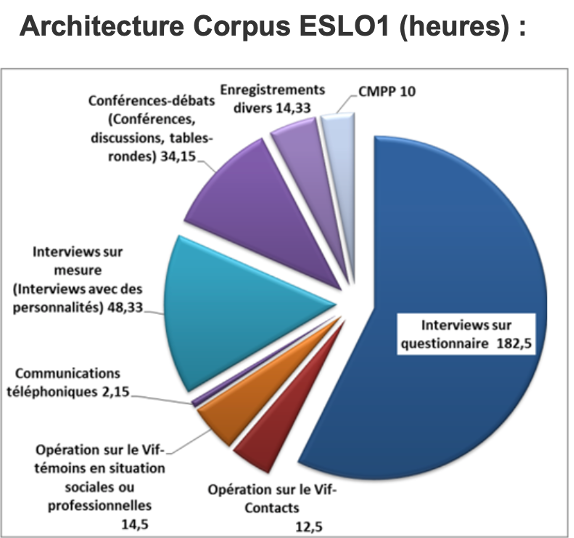
\includegraphics[width=\textwidth]{images/eslo1.png}
        %\caption{Neural Network with 5 neurons in the hidden layer. }
        \end{figure}
    \column{0.5\textwidth}

    \end{columns}
    
\end{frame}
%   FRAME END   --==-=-=-=-=-=-=-=-=-=-=-=-=-=-=-=-=-=-=-=-=-=-=-=-=-=-=-=-=-=-=
\begin{frame}[c]{The corpora}

    \noindent The corpora are composed of several different recording types:

\begin{columns}
    \column{0.5\textwidth}
        \begin{figure}
        \centering
        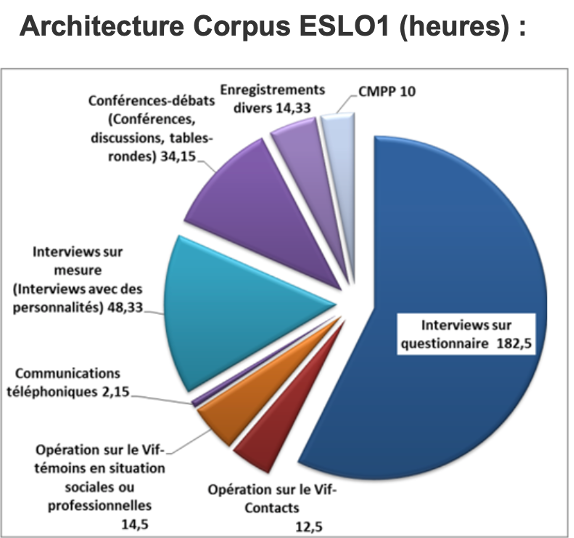
\includegraphics[width=\textwidth]{images/eslo1.png}
        %\caption{Neural Network with 5 neurons in the hidden layer. }
        \end{figure}
    \column{0.5\textwidth}
        \begin{figure}
        \centering
        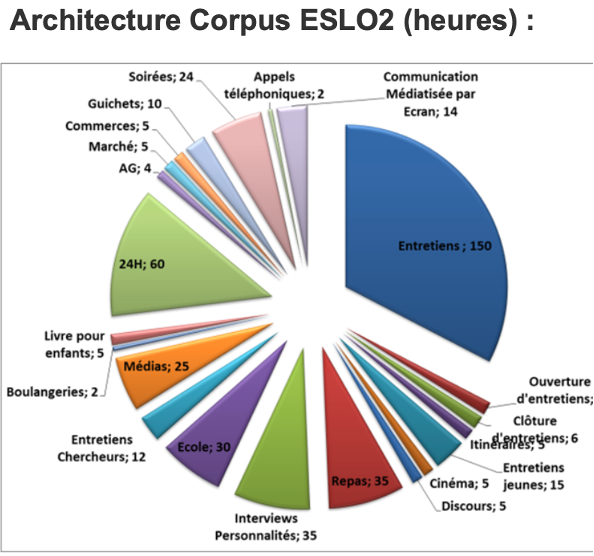
\includegraphics[width=\textwidth]{images/eslo2.png}
        %\caption{Neural Network with 5 neurons in the hidden layer. }
        \end{figure}
    \end{columns}
    
    
\end{frame}
%   FRAME END   --==-=-=-=-=-=-=-=-=-=-=-=-=-=-=-=-=-=-=-=-=-=-=-=-=-=-=-=-=-=-=
%   FRAME START   -=-=-=-=-=-=-=-=-=-=-=-=-=-=-=-=-=-=-=-=-=-=-=-=-=-=-=-=-=-=-=
\begin{frame}[c]{Data extraction}

    \transboxin<1>
    \transglitter<2>
    %\transwipe<3>
    \noindent The data was extracted using the eslo 'faire une requête dans le corpus' page. \pause

    \begin{itemize}
        \item[\ding{227}] 'mot exact' search (cvs); \pause
        \item[\ding{227}] automatic extraction of all interrogatives (the corpus is transcribed).
    \end{itemize}
    
\end{frame}
%   FRAME END   --==-=-=-=-=-=-=-=-=-=-=-=-=-=-=-=-=-=-=-=-=-=-=-=-=-=-=-=-=-=-=
%   FRAME START   -=-=-=-=-=-=-=-=-=-=-=-=-=-=-=-=-=-=-=-=-=-=-=-=-=-=-=-=-=-=-=
\begin{frame}[c]{Data classification}

    \transboxin<1>
    \transglitter<2>
    \transwipe<3>
    \noindent The data was pre-classified automatically (and then checked manually).\\ \pause
    \noindent \textbf{All} wh-in situ occurrences $+$ all questions with uncertain interpretation (genuine, echo etc.) were listened carefully by both authors.\\
    
    \textbf{\textsc{basic classification}} \pause
    \begin{enumerate}
        \item position of the wh-element \pause (ex situ, in situ); \pause
        \item interrogative strategy \pause (SV, est-ce que, VS); \pause
        \item clause-final vs clause-internal position; \pause
        \item well-formedness \pause (formed, fragment).
        \item tripartition.
    \end{enumerate}
    
\end{frame}
%   FRAME END   --==-=-=-=-=-=-=-=-=-=-=-=-=-=-=-=-=-=-=-=-=-=-=-=-=-=-=-=-=-=-=
%   FRAME START   -=-=-=-=-=-=-=-=-=-=-=-=-=-=-=-=-=-=-=-=-=-=-=-=-=-=-=-=-=-=-=
\begin{frame}[c]{Data cleaning}

    \transboxin<1>
    \transglitter<2>
    \transwipe<3>
    \textbf{\textsc{data that we considered}} \pause
    
    \begin{itemize}
        \item[\ding{227}] wh-questions \pause (as opposed to yes/no questions); \pause
        \item[\ding{227}] matrix monoclausal questions \pause (no long distance questions, no embedded questions, no infinitives, etc.); \pause
        \item[\ding{227}] real questions \pause (no rethoric questions, echo questions, quiz questions, introspective questions etc.); \pause
        \item[\ding{227}] well-formed clauses \pause (no fragments, no questions containing only a wh-element ('Qui?', 'Quoi?')); \pause
        \item[\ding{227}] utterances by French native speakers.
    \end{itemize}
    
\end{frame}
%   FRAME END   --==-=-=-=-=-=-=-=-=-=-=-=-=-=-=-=-=-=-=-=-=-=-=-=-=-=-=-=-=-=-=
\begin{frame}[c]{Data cleaning}

    \transboxin<1>
    \transglitter<2>
    \transwipe<3>
    \textbf{\textsc{which wh-elements?}} \pause
    
    \begin{itemize}
        \item[\ding{227}] we only studied non-lexically restricted wh-elements ('what?', no 'which chair?'); \pause
        \item[\ding{227}] today, I shall only present the data on those wh-elements that can surface either in situ or ex situ (e.g. not 'que'): \pause
        \begin{enumerate}
            \item quand; \pause
            \item où; \pause
            \item comment; \pause
            \item quoiO; \pause
            \item quiO.
        \end{enumerate}
    \end{itemize}
    
\end{frame}
%=-=-=-=-=-=-=-=-=-=-=-=-=-=-=-=-=-=-=-=-=-=-=-=-=-=-=-=-=-=-=-=-=-=-=-=-=-=-=-=
%   FRAME END   --==-=-=-=-=-=-=-=-=-=-=-=-=-=-=-=-=-=-=-=-=-=-=-=-=-=-=-=-=-=-=
\begin{frame}[c]{Data cleaning}


    \textbf{\textsc{which wh-elements?}}
    
    \begin{itemize}
        \item[\ding{227}] we only studied non-lexically restricted wh-elements ('what?', no 'which chair?');
        \item[\ding{227}] today, I shall only present the data on those wh-elements that can surface either in situ or ex situ (e.g. not 'que'):
        \begin{enumerate}
            \item {\st{quand}};
            \item où;
            \item comment;
            \item quoiO;
            \item {\st{quiO}}.
        \end{enumerate}
    \end{itemize}
    
\end{frame}
%=-=-=-=-=-=-=-=-=-=-=-=-=-=-=-=-=-=-=-=-=-=-=-=-=-=-=-=-=-=-=-=-=-=-=-=-=-=-=-=
\end{document}